% Đề cương ôn tập Toán 11: Lượng giác và Dãy số (một mặt A4).
% Biên dịch: xelatex de-cuong-toan-11.tex
\documentclass[10pt]{extarticle}
\usepackage[a4paper,margin=7mm,top=6mm,bottom=6mm]{geometry}
\usepackage{fontspec}
\setmainfont{Latin Modern Roman}
\newfontfamily\headfont{Inter}[UprightFont=* SemiBold,BoldFont=* ExtraBold]
\usepackage{amsmath,amssymb}
\usepackage{multicol}
\usepackage[most]{tcolorbox}
\usepackage{tikz}
\usetikzlibrary{arrows.meta,decorations.pathreplacing,calc}
\usepackage{array,booktabs}
\pagestyle{empty}
\setlength{\parindent}{0pt}
\setlength{\columnsep}{4mm}
\setlength{\abovedisplayskip}{2pt}
\setlength{\belowdisplayskip}{2pt}
\setlength{\abovedisplayshortskip}{1pt}
\setlength{\belowdisplayshortskip}{1pt}
\setlength{\jot}{1pt}

% Màu dùng chung với video: cos xanh dương, sin hồng, nhấn vàng cam
\definecolor{ink}{HTML}{1B2333}
\definecolor{cosc}{HTML}{1F7AE0}
\definecolor{sinc}{HTML}{E0365F}
\definecolor{tanc}{HTML}{0E9F7E}
\definecolor{cotc}{HTML}{7357D6}
\definecolor{key}{HTML}{E08A00}
\definecolor{soft}{HTML}{F3F6FB}
\definecolor{muted}{HTML}{5A6478}

% Hộp cho từng mục
\newtcolorbox{muc}[2][cosc]{enhanced,colback=white,colframe=#1,boxrule=0.6pt,arc=2mm,
  left=1.6mm,right=1.6mm,top=0.8mm,bottom=1mm,before skip=1.4mm,after skip=0mm,
  title={\headfont\small #2},fonttitle=\color{white},coltitle=white,
  colbacktitle=#1,toptitle=0.3mm,bottomtitle=0.3mm,unbreakable}
% Công thức đóng khung
\newcommand{\kq}[1]{\tcbox[on line,colback=key!10,colframe=key,boxrule=0.5pt,arc=1mm,
  left=1mm,right=1mm,top=0.4mm,bottom=0.4mm,boxsep=0pt]{$\displaystyle #1$}}
\newcommand{\ghi}[1]{{\color{muted}\small #1}}

\begin{document}
\color{ink}

% ---------------- Tiêu đề ----------------
\begin{tcolorbox}[enhanced,colback=ink,colframe=ink,arc=2mm,left=3mm,right=3mm,top=1.2mm,bottom=1.2mm]
\color{white}{\headfont\bfseries\large ĐỀ CƯƠNG ÔN TẬP TOÁN 11 \quad·\quad LƯỢNG GIÁC \& DÃY SỐ}
\hfill{\footnotesize Họ và tên: \makebox[30mm]{\dotfill}\ \ Lớp: \makebox[9mm]{\dotfill}}
\end{tcolorbox}

\raggedcolumns
\begin{multicols*}{3}

% ================= 1. Radian =================
\begin{muc}{1. Radian và độ dài cung}
\begin{center}\kq{180^\circ=\pi\text{ rad}}\qquad \kq{l=R|\alpha|}\end{center}
\vspace{-1mm}
\centerline{$1^\circ=\dfrac{\pi}{180}\text{ rad},\quad 1\text{ rad}=\Big(\dfrac{180}{\pi}\Big)^{\!\circ}\approx57{,}3^\circ$}\vspace{1pt}
$R$: bán kính; $\alpha$: số đo góc ở tâm tính bằng \textbf{radian}. Nếu đang dùng \textbf{độ}, phải đổi sang radian trước.\\
\ghi{VD: $R=2$, $\alpha=60^\circ=\frac{\pi}{3}\Rightarrow l=\frac{2\pi}{3}$.}
\end{muc}

% ================= 2. Giá trị lượng giác =================
\begin{muc}{2. Giá trị lượng giác của góc $\alpha$}
\begin{minipage}[c]{0.56\linewidth}
\centering
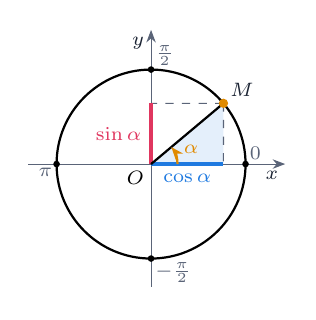
\begin{tikzpicture}[scale=1.2,>={Stealth[length=1.6mm]}]
  \draw[->,muted] (-1.3,0)--(1.42,0) node[below left=-1pt,ink]{\scriptsize$x$};
  \draw[->,muted] (0,-1.3)--(0,1.42) node[below left=-1pt,ink]{\scriptsize$y$};
  \draw[thick] (0,0) circle (1);
  \coordinate (M) at (40:1);
  \fill[cosc!12] (0,0)--(M)--({cos(40)},0)--cycle;
  \draw[dashed,muted] (M)--({cos(40)},0) (M)--(0,{sin(40)});
  \draw[cosc,line width=1.6pt] (0,0)--({cos(40)},0);
  \draw[sinc,line width=1.6pt] (0,0)--(0,{sin(40)});
  \draw[thick] (0,0)--(M);
  \draw[key,thick,->] (0.28,0) arc (0:40:0.28);
  \node[key] at (20:0.45) {\scriptsize$\alpha$};
  \fill[key] (M) circle (1.4pt) node[above right=-1pt,ink] {\scriptsize$M$};
  \node[cosc,below] at ({cos(40)/2},0) {\scriptsize$\cos\alpha$};
  \node[sinc,left] at (0,{sin(40)/2}) {\scriptsize$\sin\alpha$};
  \foreach \a/\t/\p in {0/0/above right,90/\frac{\pi}{2}/above right,180/\pi/below left,270/-\frac{\pi}{2}/below right}
    {\fill (\a:1) circle (1pt) node[\p=-2pt,muted] {\scriptsize$\t$};}
  \node[below left=-1pt] at (0,0) {\scriptsize$O$};
\end{tikzpicture}
\end{minipage}%
\begin{minipage}[c]{0.44\linewidth}
\small
{\color{cosc}$\cos\alpha=x_M$}\\ \ghi{\scriptsize(hoành độ)}\\[1pt]
{\color{sinc}$\sin\alpha=y_M$}\\ \ghi{\scriptsize(tung độ)}\\[3pt]
$\tan\alpha=\dfrac{\sin\alpha}{\cos\alpha}$\\[3pt]
$\cot\alpha=\dfrac{\cos\alpha}{\sin\alpha}$
\end{minipage}\\[1pt]
\centerline{\small $-1\le\sin\alpha\le1,\quad -1\le\cos\alpha\le1$}
\begin{center}\vspace{-1mm}\kq{\sin^2\alpha+\cos^2\alpha=1}\end{center}
\vspace{-1mm}
\ghi{Hệ quả: $1+\tan^2\alpha=\frac{1}{\cos^2\alpha}$,\ $1+\cot^2\alpha=\frac{1}{\sin^2\alpha}$,\ $\tan\alpha\cot\alpha=1$.}
\end{muc}

% ================= 3. Giá trị đặc biệt & ĐKXĐ =================
\begin{muc}{3. Khi nào sin, cos bằng 0, 1, $-1$? \ ($k\in\mathbb Z$)}
\renewcommand{\arraystretch}{1.28}
\setlength{\tabcolsep}{2pt}
\centering
\begin{tabular}{@{}r@{\ $\Leftrightarrow$\ }l@{}}
{\color{sinc}$\sin\alpha=0$} & $\alpha=k\pi$\\
{\color{sinc}$\sin\alpha=1$} & $\alpha=\frac{\pi}{2}+k2\pi$\\
{\color{sinc}$\sin\alpha=-1$} & $\alpha=-\frac{\pi}{2}+k2\pi$\\\hline
{\color{cosc}$\cos\alpha=0$} & $\alpha=\frac{\pi}{2}+k\pi$\\
{\color{cosc}$\cos\alpha=1$} & $\alpha=k2\pi$\\
{\color{cosc}$\cos\alpha=-1$} & $\alpha=\pi+k2\pi$
\end{tabular}\\[2pt]
\raggedright
\ghi{Mẹo: $\sin\alpha=0$ khi $M$ nằm trên trục hoành; $\cos\alpha=0$ khi $M$ nằm trên trục tung.}\\[3pt]
\textbf{Điều kiện xác định} (mẫu số khác 0):\\[1pt]
{\color{tanc}$\tan\alpha$}: $\cos\alpha\ne0\Leftrightarrow$ \kq{\alpha\ne\tfrac{\pi}{2}+k\pi}\\[2pt]
{\color{cotc}$\cot\alpha$}: $\sin\alpha\ne0\Leftrightarrow$ \kq{\alpha\ne k\pi}
\end{muc}

% ================= Ghi chú =================
\begin{muc}[muted]{Ghi chú}
\vspace{1mm}
\foreach \i in {1,...,7}{\makebox[\linewidth]{\color{muted!60}\dotfill}\\[2.2mm]}
\end{muc}

\columnbreak

% ================= 4. Góc liên quan đặc biệt =================
\begin{muc}{4. Giá trị lượng giác của các góc liên quan}
\centering
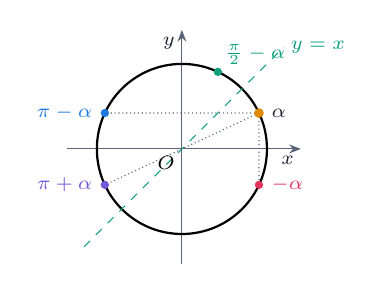
\begin{tikzpicture}[scale=1.08,>={Stealth[length=1.5mm]}]
  \draw[->,muted] (-1.35,0)--(1.4,0) node[below left=-1pt,ink]{\scriptsize$x$};
  \draw[->,muted] (0,-1.35)--(0,1.4) node[below left=-1pt,ink]{\scriptsize$y$};
  \draw[thick] (0,0) circle (1);
  \draw[dashed,tanc] (-1.15,-1.15)--(1.2,1.2) node[right=-1pt]{\scriptsize$y=x$};
  \def\a{25}
  \draw[densely dotted,muted] (\a:1)--(-\a:1) (\a:1)--(180-\a:1) (\a:1)--(180+\a:1);
  \fill[key] (\a:1) circle (1.6pt) node[right=1pt,ink]{\scriptsize$\alpha$};
  \fill[sinc] (-\a:1) circle (1.4pt) node[right=1pt]{\scriptsize$-\alpha$};
  \fill[cosc] (180-\a:1) circle (1.4pt) node[left=1pt]{\scriptsize$\pi-\alpha$};
  \fill[tanc] (90-\a:1) circle (1.4pt) node[above right=-1pt]{\scriptsize$\frac{\pi}{2}-\alpha$};
  \fill[cotc] (180+\a:1) circle (1.4pt) node[left=1pt]{\scriptsize$\pi+\alpha$};
  \node[below left=-1pt] at (0,0) {\scriptsize$O$};
\end{tikzpicture}\\[-1pt]
{\scriptsize\color{muted}đối: qua $Ox$ \ · \ bù: qua $Oy$ \ · \ phụ: qua $y=x$ \ · \ hơn kém $\pi$: qua $O$}\\[2pt]
\renewcommand{\arraystretch}{1.3}
\setlength{\tabcolsep}{1.7pt}
\setlength{\fboxsep}{0.8pt}
\small
\begin{tabular}{@{}c|c|c|c|c@{}}
 & \color{sinc}Đối & \color{cosc}Bù & \color{tanc}Phụ & \color{cotc}Hơn kém $\pi$\\[-2pt]
 & \color{sinc}$-\alpha$ & \color{cosc}$\pi-\alpha$ & \color{tanc}$\frac{\pi}{2}-\alpha$ & \color{cotc}$\pi+\alpha$\\\hline
$\sin$ & $-\sin\alpha$ & \colorbox{key!18}{$\sin\alpha$} & $\cos\alpha$ & $-\sin\alpha$\\
$\cos$ & \colorbox{key!18}{$\cos\alpha$} & $-\cos\alpha$ & $\sin\alpha$ & $-\cos\alpha$\\
$\tan$ & $-\tan\alpha$ & $-\tan\alpha$ & $\cot\alpha$ & \colorbox{key!18}{$\tan\alpha$}\\
$\cot$ & $-\cot\alpha$ & $-\cot\alpha$ & $\tan\alpha$ & \colorbox{key!18}{$\cot\alpha$}
\end{tabular}\\[3pt]
\tcbox[colback=key!10,colframe=key,boxrule=0.5pt,arc=1mm,left=1mm,right=1mm,top=0.5mm,bottom=0.5mm,before skip=1mm,after skip=0.5mm]{\small\bfseries\begin{tabular}{@{}c@{}}Cos đối · Sin bù · Phụ chéo\\ Hơn kém $\pi$: tan, cot\end{tabular}}
\ghi{Cái được nhắc tên thì giữ nguyên, còn lại đổi dấu; phụ thì đổi chéo sin$\leftrightarrow$cos, tan$\leftrightarrow$cot.}
\end{muc}

% ================= 5. Nhân đôi =================
\begin{muc}{5. Công thức nhân đôi}
\centering
\kq{\sin2a=2\sin a\cos a}\\[3pt]
\kq{\cos2a=\cos^2a-\sin^2a}\\[2pt]
$\phantom{\cos2a}=2\cos^2a-1=1-2\sin^2a$\\[2pt]
\raggedright\ghi{(thay $\sin^2a=1-\cos^2a$ hoặc $\cos^2a=1-\sin^2a$)\\
Hạ bậc: $\cos^2a=\frac{1+\cos2a}{2}$,\ \ $\sin^2a=\frac{1-\cos2a}{2}$.}
\end{muc}

% ================= 6. Chẵn, lẻ, tuần hoàn =================
\begin{muc}{6. Hàm số chẵn, lẻ, tuần hoàn}
\begin{minipage}[t]{0.49\linewidth}\centering
\textbf{Chẵn:} $f(-x)=f(x)$\\
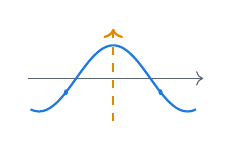
\begin{tikzpicture}[xscale=0.3,yscale=0.42]
  \draw[->,muted] (-3.6,0)--(3.8,0); \draw[->,key,thick,dashed] (0,-1.3)--(0,1.5);
  \draw[cosc,thick,domain=-3.5:3.5,samples=60] plot (\x,{cos(\x r)});
  \fill[cosc] (2,{cos(2 r)}) circle (2.5pt) (-2,{cos(2 r)}) circle (2.5pt);
\end{tikzpicture}\\
\scriptsize đối xứng qua \textbf{trục tung}\\ VD: $\cos x$, $x^2$
\end{minipage}\hfill
\begin{minipage}[t]{0.49\linewidth}\centering
\textbf{Lẻ:} $f(-x)=-f(x)$\\
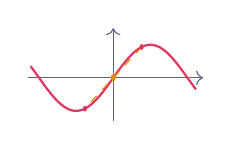
\begin{tikzpicture}[xscale=0.3,yscale=0.42]
  \draw[->,muted] (-3.6,0)--(3.8,0); \draw[->,muted] (0,-1.3)--(0,1.5);
  \draw[sinc,thick,domain=-3.5:3.5,samples=60] plot (\x,{sin(\x r)});
  \draw[key,dashed] (1.2,{sin(1.2 r)})--(-1.2,{-sin(1.2 r)});
  \fill[key] (0,0) circle (3pt);
  \fill[sinc] (1.2,{sin(1.2 r)}) circle (2.5pt) (-1.2,{-sin(1.2 r)}) circle (2.5pt);
\end{tikzpicture}\\
\scriptsize đối xứng qua \textbf{gốc tọa độ}\\ VD: $\sin x$, $\tan x$, $x^3$
\end{minipage}\\[2pt]
\ghi{Cả hai đều cần: $x\in D\Rightarrow -x\in D$.}\\[3pt]
\textbf{Tuần hoàn:} $f$ tuần hoàn nếu tồn tại $T>0$ sao cho
\begin{center}\vspace{-1.5mm}\kq{f(x+T)=f(x),\ \forall x\in D}\end{center}
\vspace{-1mm}
và $x+T\in D$ với mọi $x\in D$.\\[1pt]
\centering
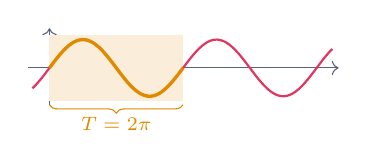
\begin{tikzpicture}[xscale=0.27,yscale=0.36]
  \draw[->,muted] (-1,0)--(13.6,0); \draw[->,muted] (0,-1.3)--(0,1.4);
  \fill[key!15] (0,-1.15) rectangle ({2*pi},1.15);
  \draw[sinc,thick,domain=-0.8:13.3,samples=100] plot (\x,{sin(\x r)});
  \draw[key,very thick,domain=0:{2*pi},samples=50] plot (\x,{sin(\x r)});
  \draw[decorate,decoration={brace,amplitude=3pt,mirror},key] (0,-1.3)--({2*pi},-1.3) node[midway,below=1pt]{\scriptsize$T=2\pi$};
\end{tikzpicture}\\
\scriptsize Chu kì: $\sin,\cos$: $T=2\pi$;\quad $\tan,\cot$: $T=\pi$.
\end{muc}

\columnbreak

% ================= 7. Cấp số cộng =================
\begin{muc}[tanc]{7. Cấp số cộng (công sai $d$)}
Mỗi số hạng, kể từ số hạng thứ hai, bằng số hạng đứng ngay trước nó cộng với một số không đổi $d$:
\begin{center}\vspace{-1.5mm}\kq{u_{n+1}=u_n+d}\end{center}
\begin{minipage}[c]{0.6\linewidth}
\textbf{Số hạng tổng quát:}\\[1pt]
\kq{u_n=u_1+(n-1)d}\\[3pt]
Biết $u_m$:\\[1pt]
\kq{u_n=u_m+(n-m)d}
\end{minipage}%
\begin{minipage}[c]{0.4\linewidth}\centering
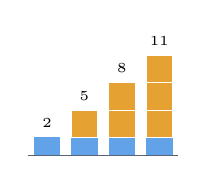
\begin{tikzpicture}[x=3.4mm,y=1.15mm]
  \foreach \i/\v in {0/2,1/5,2/8,3/11}{
    \fill[cosc!70] (\i*1.4,0) rectangle ++(1,2);
    \pgfmathtruncatemacro{\k}{\i}
    \ifnum\k>0 \foreach \j in {1,...,\k}{\fill[key!80,draw=white,line width=0.3pt] (\i*1.4,{2+3*(\j-1)}) rectangle ++(1,3);}\fi
    \node[above,font=\tiny] at (\i*1.4+0.5,\v) {$\v$};
  }
  \draw[muted] (-0.2,0)--(5.4,0);
\end{tikzpicture}\\[-1pt]
{\scriptsize{\color{cosc}$\blacksquare$}\,$u_1$\ \ {\color{key}$\blacksquare$}\,$d$}
\end{minipage}\\[3pt]
\textbf{Tổng $n$ số hạng đầu:}
\begin{center}\vspace{-1.5mm}
\kq{S_n=\frac{n}{2}\big[2u_1+(n-1)d\big]}\\[3pt]
\kq{S_n=\frac{n(u_1+u_n)}{2}}
\end{center}
\vspace{-1mm}
\ghi{VD: $2+5+8+11+14=\frac{5(2+14)}{2}=40$.}\\
\ghi{Ba số $a,b,c$ lập CSC $\Leftrightarrow a+c=2b$.}
\end{muc}

% ================= 8. Cấp số nhân =================
\begin{muc}[cotc]{8. Cấp số nhân (công bội $q$)}
Mỗi số hạng, kể từ số hạng thứ hai, bằng số hạng đứng ngay trước nó nhân với một số không đổi $q$:
\begin{center}\vspace{-1.5mm}\kq{u_{n+1}=u_n\cdot q}\end{center}
\begin{minipage}[c]{0.6\linewidth}
\textbf{Số hạng tổng quát:}\\[1pt]
\kq{u_n=u_1q^{n-1}}\\[3pt]
Biết $u_m$:\\[1pt]
\kq{u_n=u_mq^{n-m}}
\end{minipage}%
\begin{minipage}[c]{0.4\linewidth}\centering
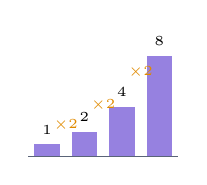
\begin{tikzpicture}[x=3.4mm,y=1.6mm]
  \foreach \i/\v in {0/1,1/2,2/4,3/8}{
    \fill[cotc!75,draw=white,line width=0.3pt] (\i*1.4,0) rectangle ++(1,\v);
    \node[above,font=\tiny] at (\i*1.4+0.5,\v) {$\v$};
  }
  \foreach \i in {1,2,3}{\node[font=\tiny,key] at (\i*1.4-0.2,{2^(\i-1)+0.9+\i*0.6}) {$\times2$};}
  \draw[muted] (-0.2,0)--(5.4,0);
\end{tikzpicture}\\[-1pt]
{\scriptsize\color{key}cột sau gấp $q$ lần}
\end{minipage}\\[3pt]
\textbf{Tổng $n$ số hạng đầu} (với $q\ne1$):
\begin{center}\vspace{-1.5mm}
\kq{S_n=\frac{u_1(1-q^n)}{1-q}}\ \ hay\ \ \kq{S_n=\frac{u_1(q^n-1)}{q-1}}
\end{center}
\vspace{-1mm}
\ghi{Nếu $q=1$ thì $S_n=nu_1$.\quad VD: $1+2+4+8+16=\frac{2^5-1}{2-1}=31$.}\\
\ghi{Ba số $a,b,c$ lập CSN $\Leftrightarrow b^2=ac$.}
\end{muc}

% ================= 9. Bảng giá trị đặc biệt =================
\begin{muc}[key]{9. Giá trị lượng giác của các góc đặc biệt}
\centering\small
\renewcommand{\arraystretch}{1.45}
\setlength{\tabcolsep}{3.2pt}
\begin{tabular}{@{}c|ccccc@{}}
$\alpha$ & $0$ & $\frac{\pi}{6}$ & $\frac{\pi}{4}$ & $\frac{\pi}{3}$ & $\frac{\pi}{2}$\\
 & \scriptsize$0^\circ$ & \scriptsize$30^\circ$ & \scriptsize$45^\circ$ & \scriptsize$60^\circ$ & \scriptsize$90^\circ$\\\hline
\color{sinc}$\sin$ & $0$ & $\frac12$ & $\frac{\sqrt2}{2}$ & $\frac{\sqrt3}{2}$ & $1$\\
\color{cosc}$\cos$ & $1$ & $\frac{\sqrt3}{2}$ & $\frac{\sqrt2}{2}$ & $\frac12$ & $0$\\
\color{tanc}$\tan$ & $0$ & $\frac{\sqrt3}{3}$ & $1$ & $\sqrt3$ & \color{muted}\scriptsize k.x.đ\\
\color{cotc}$\cot$ & \color{muted}\scriptsize k.x.đ & $\sqrt3$ & $1$ & $\frac{\sqrt3}{3}$ & $0$
\end{tabular}\\[2pt]
\raggedright\ghi{k.x.đ: không xác định. Đọc $\sin$ từ trái sang phải giống $\cos$ từ phải sang trái (góc phụ nhau).}
\end{muc}

\end{multicols*}
\end{document}
